\documentclass[]{article}
\usepackage{lmodern}
\usepackage{amssymb,amsmath}
\usepackage{ifxetex,ifluatex}
\usepackage{fixltx2e} % provides \textsubscript
\ifnum 0\ifxetex 1\fi\ifluatex 1\fi=0 % if pdftex
  \usepackage[T1]{fontenc}
  \usepackage[utf8]{inputenc}
\else % if luatex or xelatex
  \ifxetex
    \usepackage{mathspec}
  \else
    \usepackage{fontspec}
  \fi
  \defaultfontfeatures{Ligatures=TeX,Scale=MatchLowercase}
\fi
% use upquote if available, for straight quotes in verbatim environments
\IfFileExists{upquote.sty}{\usepackage{upquote}}{}
% use microtype if available
\IfFileExists{microtype.sty}{%
\usepackage{microtype}
\UseMicrotypeSet[protrusion]{basicmath} % disable protrusion for tt fonts
}{}
\usepackage[margin=1in]{geometry}
\usepackage{hyperref}
\hypersetup{unicode=true,
            pdftitle={Introduction to R},
            pdfauthor={Allison Theobold \& The Carpentries},
            pdfborder={0 0 0},
            breaklinks=true}
\urlstyle{same}  % don't use monospace font for urls
\usepackage{color}
\usepackage{fancyvrb}
\newcommand{\VerbBar}{|}
\newcommand{\VERB}{\Verb[commandchars=\\\{\}]}
\DefineVerbatimEnvironment{Highlighting}{Verbatim}{commandchars=\\\{\}}
% Add ',fontsize=\small' for more characters per line
\usepackage{framed}
\definecolor{shadecolor}{RGB}{248,248,248}
\newenvironment{Shaded}{\begin{snugshade}}{\end{snugshade}}
\newcommand{\KeywordTok}[1]{\textcolor[rgb]{0.13,0.29,0.53}{\textbf{#1}}}
\newcommand{\DataTypeTok}[1]{\textcolor[rgb]{0.13,0.29,0.53}{#1}}
\newcommand{\DecValTok}[1]{\textcolor[rgb]{0.00,0.00,0.81}{#1}}
\newcommand{\BaseNTok}[1]{\textcolor[rgb]{0.00,0.00,0.81}{#1}}
\newcommand{\FloatTok}[1]{\textcolor[rgb]{0.00,0.00,0.81}{#1}}
\newcommand{\ConstantTok}[1]{\textcolor[rgb]{0.00,0.00,0.00}{#1}}
\newcommand{\CharTok}[1]{\textcolor[rgb]{0.31,0.60,0.02}{#1}}
\newcommand{\SpecialCharTok}[1]{\textcolor[rgb]{0.00,0.00,0.00}{#1}}
\newcommand{\StringTok}[1]{\textcolor[rgb]{0.31,0.60,0.02}{#1}}
\newcommand{\VerbatimStringTok}[1]{\textcolor[rgb]{0.31,0.60,0.02}{#1}}
\newcommand{\SpecialStringTok}[1]{\textcolor[rgb]{0.31,0.60,0.02}{#1}}
\newcommand{\ImportTok}[1]{#1}
\newcommand{\CommentTok}[1]{\textcolor[rgb]{0.56,0.35,0.01}{\textit{#1}}}
\newcommand{\DocumentationTok}[1]{\textcolor[rgb]{0.56,0.35,0.01}{\textbf{\textit{#1}}}}
\newcommand{\AnnotationTok}[1]{\textcolor[rgb]{0.56,0.35,0.01}{\textbf{\textit{#1}}}}
\newcommand{\CommentVarTok}[1]{\textcolor[rgb]{0.56,0.35,0.01}{\textbf{\textit{#1}}}}
\newcommand{\OtherTok}[1]{\textcolor[rgb]{0.56,0.35,0.01}{#1}}
\newcommand{\FunctionTok}[1]{\textcolor[rgb]{0.00,0.00,0.00}{#1}}
\newcommand{\VariableTok}[1]{\textcolor[rgb]{0.00,0.00,0.00}{#1}}
\newcommand{\ControlFlowTok}[1]{\textcolor[rgb]{0.13,0.29,0.53}{\textbf{#1}}}
\newcommand{\OperatorTok}[1]{\textcolor[rgb]{0.81,0.36,0.00}{\textbf{#1}}}
\newcommand{\BuiltInTok}[1]{#1}
\newcommand{\ExtensionTok}[1]{#1}
\newcommand{\PreprocessorTok}[1]{\textcolor[rgb]{0.56,0.35,0.01}{\textit{#1}}}
\newcommand{\AttributeTok}[1]{\textcolor[rgb]{0.77,0.63,0.00}{#1}}
\newcommand{\RegionMarkerTok}[1]{#1}
\newcommand{\InformationTok}[1]{\textcolor[rgb]{0.56,0.35,0.01}{\textbf{\textit{#1}}}}
\newcommand{\WarningTok}[1]{\textcolor[rgb]{0.56,0.35,0.01}{\textbf{\textit{#1}}}}
\newcommand{\AlertTok}[1]{\textcolor[rgb]{0.94,0.16,0.16}{#1}}
\newcommand{\ErrorTok}[1]{\textcolor[rgb]{0.64,0.00,0.00}{\textbf{#1}}}
\newcommand{\NormalTok}[1]{#1}
\usepackage{graphicx,grffile}
\makeatletter
\def\maxwidth{\ifdim\Gin@nat@width>\linewidth\linewidth\else\Gin@nat@width\fi}
\def\maxheight{\ifdim\Gin@nat@height>\textheight\textheight\else\Gin@nat@height\fi}
\makeatother
% Scale images if necessary, so that they will not overflow the page
% margins by default, and it is still possible to overwrite the defaults
% using explicit options in \includegraphics[width, height, ...]{}
\setkeys{Gin}{width=\maxwidth,height=\maxheight,keepaspectratio}
\IfFileExists{parskip.sty}{%
\usepackage{parskip}
}{% else
\setlength{\parindent}{0pt}
\setlength{\parskip}{6pt plus 2pt minus 1pt}
}
\setlength{\emergencystretch}{3em}  % prevent overfull lines
\providecommand{\tightlist}{%
  \setlength{\itemsep}{0pt}\setlength{\parskip}{0pt}}
\setcounter{secnumdepth}{0}
% Redefines (sub)paragraphs to behave more like sections
\ifx\paragraph\undefined\else
\let\oldparagraph\paragraph
\renewcommand{\paragraph}[1]{\oldparagraph{#1}\mbox{}}
\fi
\ifx\subparagraph\undefined\else
\let\oldsubparagraph\subparagraph
\renewcommand{\subparagraph}[1]{\oldsubparagraph{#1}\mbox{}}
\fi

%%% Use protect on footnotes to avoid problems with footnotes in titles
\let\rmarkdownfootnote\footnote%
\def\footnote{\protect\rmarkdownfootnote}

%%% Change title format to be more compact
\usepackage{titling}

% Create subtitle command for use in maketitle
\providecommand{\subtitle}[1]{
  \posttitle{
    \begin{center}\large#1\end{center}
    }
}

\setlength{\droptitle}{-2em}

  \title{Introduction to R}
    \pretitle{\vspace{\droptitle}\centering\huge}
  \posttitle{\par}
    \author{Allison Theobold \& The Carpentries}
    \preauthor{\centering\large\emph}
  \postauthor{\par}
    \date{}
    \predate{}\postdate{}
  

\begin{document}
\maketitle

The term \texttt{R} is used to refer to both the programming language as
well as the software that interprets the scripts written using it. The
learning curve may besteeper than with other statistical software, but
with \texttt{R} the results of youranalysis or your plot does not rely
on remembering what order you clicked on things, but instead on the
written commands you generated. In \texttt{R} you will work in scripts
or with dynamic documents, with scripts within them (Rmd or Rnw files).
Scripts may feel strange at first, but they make the steps you used in
your analysis clear for both you and for someone who wants to give you
feedback, further promoting the importance of reproducible science!

RStudio is a free computer application that allows you access to the
resources of \texttt{R}, while providing you with a comfortable working
environment. There are many ways you can interact with \texttt{R}, but
for many reasons RStudio has become the most popular. To function
correctly, RStudio uses \texttt{R} behind the scenes, hence both need to
be installed on your computer. Both \texttt{R} and \texttt{RStudio} are
cross-platform, so that everyone's versions look and operate the same
regardless of their operating system!

For our workshop, we will be making use of the RStudio Cloud. The
RStudio Cloud functions and looks the same as the RStudio you can
install on your computer, but comes with some perks for collaboration
and easily accessing the workshop materials. If you so wish, you can
choose to download a local copy of RStudio on your personal computer.
There are many videos and guides for installation. See the Stat 217
textbook (pages 12-14) here:
\url{https://scholarworks.montana.edu/xmlui/bitstream/handle/1/2999/Greenwood_Book.pdf?sequence=3\&isAllowed=y_}

RStudio has a panel of 4 windows, where each can be viewed at the same
time and has multiple tabs available.

\begin{itemize}
\tightlist
\item
  the \textbf{Editor} for your scripts and documents (top-left)\\
\item
  the \texttt{R} \textbf{Console} (bottom-left)\\
\item
  your \textbf{Environment (Objects/Variables)/History} (top-right)\\
\item
  and your \textbf{Files/Plots/Packages/Help/Viewer} (bottom-right).
\end{itemize}

\begin{figure}
\centering
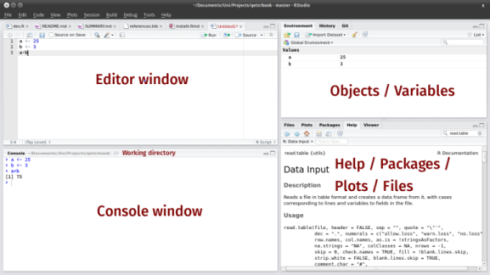
\includegraphics{images/rstudio.png}
\caption{}
\end{figure}

\newpage 

\section{\texorpdfstring{Work Flow in
\texttt{R}}{Work Flow in R}}\label{work-flow-in-r}

Many people tend to organize their projects like this:

\begin{figure}
\centering
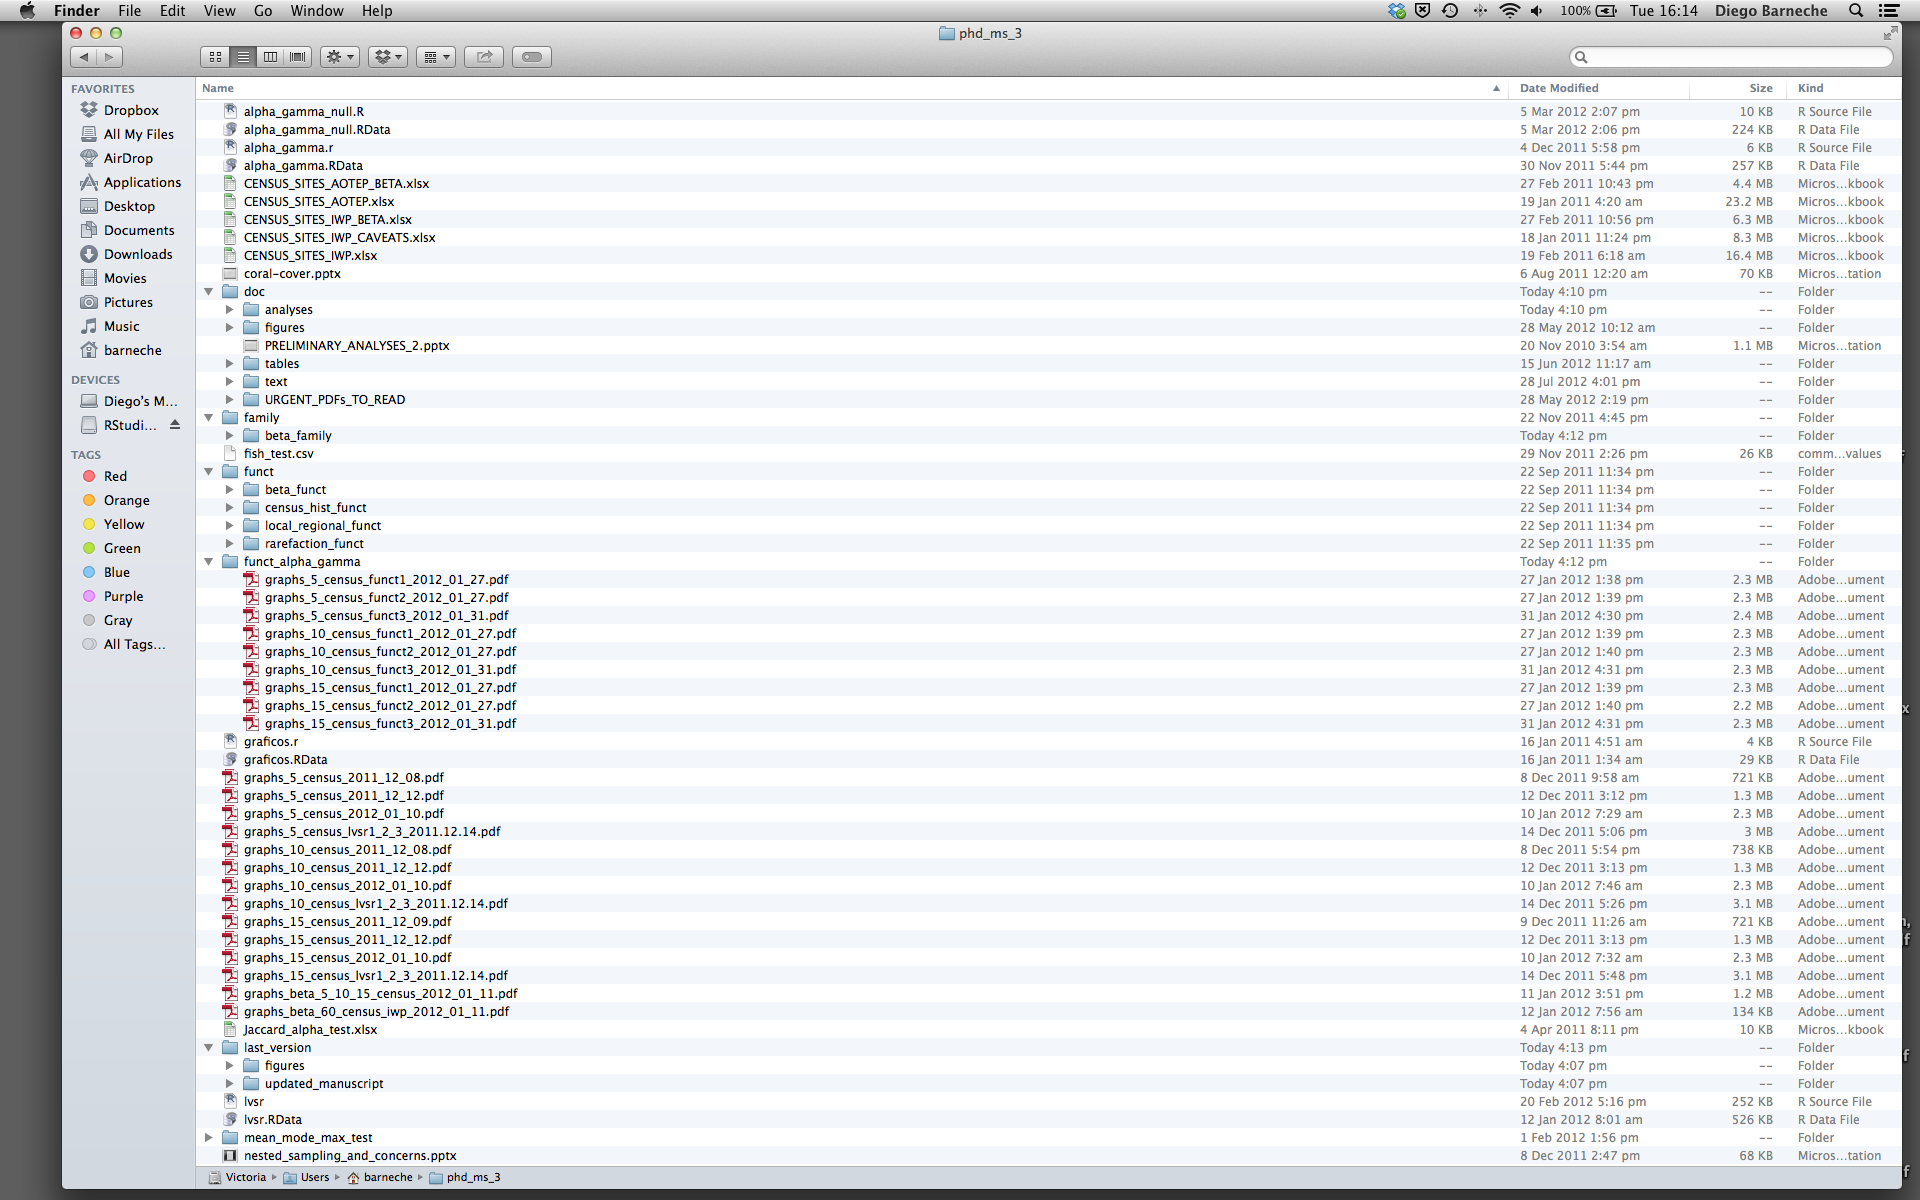
\includegraphics{images/bad_layout.png}
\caption{}
\end{figure}

There are many reasons we should \emph{always} avoid this shamble of
organization:

\begin{itemize}
\tightlist
\item
  it is really hard to tell which version of your data is original and
  what versions are modified\\
\item
  things get really messy because all types of files are mixed
  together\\
\item
  it's probably hard for you to find things and relate the correct files
  to their respective output
\end{itemize}

Ultimately, good project organization will make your life easier! It
helps ensure the integrity of your data, makes it simpler to share your
code or get help with your code, allows for you know exactly what code
you used on a paper, and it's easier to pick a project back up.

It is good code writing and file storage practice to keep a set of all
related data, analysis, plots, documents, etc. in the same folder.
RStudio makes this process easy with the invention of projects. In an
RStudio project, all of the all the project's pieces are in the same
folder. This allows for a clean workflow and a simple working directory
for \texttt{R}. When you are executing code for a document/script
\texttt{R} will search for things (such as data) in the \underline{same}
folder as the document/script, which is called a \emph{relative path}.

The easiest way to do this is, whenever you start working on a new
project in RStudio,

\begin{enumerate}
\def\labelenumi{\arabic{enumi}.}
\tightlist
\item
  Click on the ``File'' menu button, then select ``New Project''
\item
  Click ``New Directory''\\
\item
  Click ``New Project''\\
\item
  Create a name for your project (make it explanatory!)\\
\item
  Select where the project should live\\
\item
  Click the ``Create Project'' button\\
\item
  Open the project!
\end{enumerate}

After this process \texttt{R} will be searching for objects (such as
data) in the \underline{same} folder as the project. This allows for us
to keep all of our files in a self-contained system.

\section{\texorpdfstring{Working in
\texttt{R}}{Working in R}}\label{working-in-r}

RStudio allows for you to execute commands directly from the code chunk
in the document by using the \textbf{Ctrl + Enter} (on Macs, \textbf{Cmd
+ Return}) shortcut. If you place your cursor on the line in the code
chunk that you would like to run and hit this shortcut, R will execute
that line(s) of code for you. Alternatively, you can also execute code
in the console (where the output of the commands pops up). The
difference between running code in the console and in the document is
that any code you execute in the console will be lost once you close
your \texttt{R} session. If you type code into the document's code
chunks, it will be saved when you close your \texttt{R} session. Because
we want to be able to go back and re-run our code after today's
workshop, it is better to type the command we want \texttt{R} to run in
the document and save it!

If R is ready to accept commands, the \texttt{R} console (in the
bottom-left) will show a \texttt{\textgreater{}} prompt. When \texttt{R}
receives a command (by typing, copy-pasting, or using the shortcut), it
will execute it, and when finished will display the results and show the
\texttt{\textgreater{}} symbol once again. If \texttt{R} is still
waiting for you to provide it with additional instructions, a \texttt{+}
will appear in the console. This should tell you that you didn't finish
your command. You could have forgotten to close your parenthesis or a
quotation. If this happens and you are unsure of what went wrong, click
inside the console and hit the \texttt{Esc} key. Then you can start over
and figure out where you went wrong!

\subsection{Calculator}\label{calculator}

\textbf{Practice}: Enter each of the following commands and confirm that
the response is the correct answer.

\vspace{0.25cm}

\begin{Shaded}
\begin{Highlighting}[]
\DecValTok{1} \OperatorTok{+}\StringTok{ }\DecValTok{2}

\DecValTok{16} \OperatorTok{*}\StringTok{ }\DecValTok{9}

\KeywordTok{sqrt}\NormalTok{(}\DecValTok{2}\NormalTok{)}

\DecValTok{20}\OperatorTok{/}\DecValTok{5}

\FloatTok{18.5} \OperatorTok{-}\StringTok{ }\FloatTok{7.21}

\DecValTok{3}\OperatorTok\DecValTok{2}\NormalTok{  ## what is this doing?}
\end{Highlighting}
\end{Shaded}

\section{Creating Objects}\label{creating-objects}

These operations, however, are not very interesting. To do more useful
things in \texttt{R}, we need to assign values to an object. To create
an object, we tell \texttt{R} the object's name, followed by an
assignment arrow (\texttt{\textless{}-}), and finally the value of the
object. This would look something like this:

\texttt{x\ \textless{}-\ 6}

Once we execute/run this line of code, we notice that a new object
appears in our environment window. This window shows all of the objects
that you have created during your \texttt{R} session. The value of
\texttt{x} appears next to it, since it is a scalar.

\textbf{Remarks:}

\begin{itemize}
\item
  In the above code \texttt{\textless{}-} is the assignment operator. It
  assigns values on the right to objects on the left. So, after
  executing \texttt{year\ \textless{}-\ 6}, the value of \texttt{year}
  is \texttt{6}. The arrow can be read as \texttt{6} goes into
  \texttt{year}. For historical reasons, you can also use = for
  assignments, but not in every context. Because of the slight
  differences in syntax, it is good practice to always use
  \texttt{\textless{}-} for assignments.

  \begin{itemize}
  \tightlist
  \item
    In RStudio, typing Alt at the same time as the - key will write
    \texttt{\textless{}-} in a single keystroke. Neat!
  \end{itemize}
\item
  There are a few simple rules that apply when creating the same of a
  new object (like we did above):

  \begin{itemize}
  \tightlist
  \item
    \texttt{R} is case sensitive, so if you name your variable
    \texttt{cat} but then try to run the code \texttt{Cat\ +\ 2}, you
    will get an error saying that \texttt{Cat} does not exist\\
  \item
    You also want your object's name to be explanatory, but not too
    long. Think \texttt{current\_temperature} verses
    \texttt{current\_temp}. Do you really want to type out temperature
    every time?\\
  \item
    Finally, you cannot begin any object's name with a number. You can
    end a name with a number (e.g.~clean\_data2), but does that give you
    much information about what is in the contents of
    \texttt{clean\_data2} relative to \texttt{clean\_data}?\\
  \item
    The name cannot contain any punctuation symbols, except for
    \texttt{.} and \texttt{\_} (\texttt{.} is not recommended)\\
  \item
    You should not name your object the same as any common functions you
    may use (\texttt{mean}, \texttt{sd,} etc.)
  \end{itemize}
\end{itemize}

\subsection{Clean Code}\label{clean-code}

Yes, writing code may be completely new to you, but there is a
difference between code that looks nice and code that does not.
Generally, object names should be nouns and function names should be
verbs. It is also important that your code looks presentable, so that a
friend/college/professor can read it and understand what you are doing.
For these reasons, there are style guides for writing code in
\texttt{R}. The two main style guides are Google's
\href{https://google.github.io/styleguide/Rguide.xml}{(link)} and the
slightly more comprehensive Tidyverse style guide
\href{https://style.tidyverse.org/}{(link)}. Optionally, you can install
\texttt{lintr} to automatically check and correct for issues in your
code styling. More on packages to come!

\section{Working with Objects}\label{working-with-objects}

When you assign a value to an object (like we did previously) \texttt{R}
does not output anything by default. If you enclose the code you wrote
in parenthesis, then \texttt{R} will output the value of the object you
created.

\vspace{0.25cm}

\begin{Shaded}
\begin{Highlighting}[]
\NormalTok{(x <-}\StringTok{ }\DecValTok{6}\NormalTok{)}
\end{Highlighting}
\end{Shaded}

\begin{verbatim}
## [1] 6
\end{verbatim}

\vspace{0.25cm}

Once the object has been created, you can use it! Run the following
lines of code:

\vspace{0.25cm}

\begin{Shaded}
\begin{Highlighting}[]
\FloatTok{2.2} \OperatorTok{*}\StringTok{ }\NormalTok{x}
\end{Highlighting}
\end{Shaded}

\begin{verbatim}
## [1] 13.2
\end{verbatim}

\begin{Shaded}
\begin{Highlighting}[]
\DecValTok{4} \OperatorTok{+}\StringTok{ }\NormalTok{x}
\end{Highlighting}
\end{Shaded}

\begin{verbatim}
## [1] 10
\end{verbatim}

\begin{Shaded}
\begin{Highlighting}[]
\NormalTok{x}\OperatorTok\DecValTok{3}
\end{Highlighting}
\end{Shaded}

\begin{verbatim}
## [1] 0
\end{verbatim}

\vspace{0.25cm}

We can also overwrite an object's value, so that it has a new value. In
the code below we give \texttt{x} a new value of 2 and use that to
create a new object \texttt{y}.

\vspace{0.25cm}

\begin{Shaded}
\begin{Highlighting}[]
\NormalTok{x <-}\StringTok{ }\DecValTok{2}

\NormalTok{y <-}\StringTok{ }\NormalTok{x }\OperatorTok{+}\StringTok{ }\DecValTok{6}
\end{Highlighting}
\end{Shaded}

\vspace{0.25cm}

\textbf{Exercise 1:} Change the value of \texttt{x} to back to 6 and see
what the value of \texttt{y} is. Did it change from before?

\section{Working with Different Data
Types}\label{working-with-different-data-types}

A vector is the basic data type in \texttt{R}. A vector is a series of
values, which can be either numbers or characters, but every entry of
the vector must be the same data type. \texttt{R} can tell that you are
building a vector when you use the \texttt{c()} function, which
concatenates a series of entries together.

\vspace{0.25cm}

\begin{Shaded}
\begin{Highlighting}[]
\NormalTok{temps <-}\StringTok{ }\KeywordTok{c}\NormalTok{(}\DecValTok{50}\NormalTok{, }\DecValTok{55}\NormalTok{, }\DecValTok{60}\NormalTok{, }\DecValTok{65}\NormalTok{)}
\NormalTok{temps}
\end{Highlighting}
\end{Shaded}

\begin{verbatim}
## [1] 50 55 60 65
\end{verbatim}

\vspace{0.25cm}

To make a vector of characters, you are required to use quotation marks
(" ``) to indicate to \texttt{R} that the value you are using is not an
object.

\vspace{0.25cm}

\begin{Shaded}
\begin{Highlighting}[]
\NormalTok{animals <-}\StringTok{ }\KeywordTok{c}\NormalTok{(}\StringTok{"cat"}\NormalTok{, }\StringTok{"dog"}\NormalTok{, }\StringTok{"bird"}\NormalTok{, }\StringTok{"fish"}\NormalTok{)}
\NormalTok{animals}
\end{Highlighting}
\end{Shaded}

\begin{verbatim}
## [1] "cat"  "dog"  "bird" "fish"
\end{verbatim}

\vspace{0.25cm}

Important features of a vector is the type of data they store. Run the
following lines of code and decide what type of data the vectors
contain.

\vspace{0.25cm}

\begin{Shaded}
\begin{Highlighting}[]
\KeywordTok{class}\NormalTok{(temps)}

\KeywordTok{class}\NormalTok{(animals)}
\end{Highlighting}
\end{Shaded}

\vspace{0.25cm}

\textbf{Exercise 2:} Create a vector that contains decimal valued
numbers. Then check what data type does that vector contain?

\begin{Shaded}
\begin{Highlighting}[]
\CommentTok{# Exercise 2 code here!}
\end{Highlighting}
\end{Shaded}

\newpage

Another possible data type is a logical (Boolean) value. This type of
data\\
takes on values of \texttt{TRUE} and \texttt{FALSE}. But, we said that
vectors could only be numbers or characters. If \texttt{TRUE} and
\texttt{FALSE} don't have quotations around them, then they aren't
characters. So, then they must be numbers. What numbers do you think
they are?

\vspace{0.25cm}

\begin{Shaded}
\begin{Highlighting}[]
\NormalTok{logic <-}\StringTok{ }\KeywordTok{c}\NormalTok{(}\OtherTok{TRUE}\NormalTok{, }\OtherTok{FALSE}\NormalTok{, }\OtherTok{FALSE}\NormalTok{, }\OtherTok{TRUE}\NormalTok{)}

\KeywordTok{class}\NormalTok{(logic)}
\end{Highlighting}
\end{Shaded}

\begin{verbatim}
## [1] "logical"
\end{verbatim}

\vspace{0.25cm}

\textbf{Exercise 3:} What happens when we try to mix different data
types into one vector? Speculate what will happen when we run each of
the following lines of code:

\vspace{0.25cm}

\begin{Shaded}
\begin{Highlighting}[]
\NormalTok{num_char <-}\StringTok{ }\KeywordTok{c}\NormalTok{(}\DecValTok{1}\NormalTok{, }\DecValTok{2}\NormalTok{, }\DecValTok{3}\NormalTok{, }\StringTok{"a"}\NormalTok{)}

\NormalTok{num_logic <-}\StringTok{ }\KeywordTok{c}\NormalTok{(}\DecValTok{1}\NormalTok{, }\DecValTok{2}\NormalTok{, }\DecValTok{3}\NormalTok{, }\OtherTok{FALSE}\NormalTok{)}

\NormalTok{char_logic <-}\StringTok{ }\KeywordTok{c}\NormalTok{(}\StringTok{"a"}\NormalTok{, }\StringTok{"b"}\NormalTok{, }\StringTok{"c"}\NormalTok{, }\OtherTok{TRUE}\NormalTok{)}

\NormalTok{guess <-}\StringTok{ }\KeywordTok{c}\NormalTok{(}\DecValTok{1}\NormalTok{, }\DecValTok{2}\NormalTok{, }\DecValTok{3}\NormalTok{, }\StringTok{"4"}\NormalTok{)}
\end{Highlighting}
\end{Shaded}

\vspace{0.25cm}

In each of these vectors, the two types of data were \emph{coerced} into
a single data type. This happens in a hierarchy, where some data types
get preference over others. Can we draw a diagram of the hierarchy?

\section{Lists}\label{lists}

While the elements of vectors have to be of the same data type, a list
is a special vector in \texttt{R} that allows for you to store a variety
of types of objects. If you have a vector, a matrix, a character, you
can store all of them into one list object!

The arguments to the list function are the components of the list. Where
the components can be characters, vectors, matrices, or other data
structures. Here, we create a list whose components are the three
vectors we've been working with:

\vspace{0.25cm}

\begin{Shaded}
\begin{Highlighting}[]
\NormalTok{my_first_list <-}\StringTok{ }\KeywordTok{list}\NormalTok{(animals, temps, logic)}
\NormalTok{my_first_list}
\end{Highlighting}
\end{Shaded}

\begin{verbatim}
## [[1]]
## [1] "cat"  "dog"  "bird" "fish"
## 
## [[2]]
## [1] 50 55 60 65
## 
## [[3]]
## [1]  TRUE FALSE FALSE  TRUE
\end{verbatim}

\vspace{0.25cm}

We notice that when printing a list, the output looks a bit different.
There are a whole bunch of brackets! Let's break them down. I like to
think of a list as a shelf with cubby holes. The cubby holes are the
components of the list, but there are elements in each cubby.

\begin{itemize}
\tightlist
\item
  To get to a specific component (cubby) of a list, you use the double
  brackets next to the name of the list (e.g
  \texttt{my\_first\_list{[}{[}1{]}{]}}).\\
\item
  To access the elements inside each cubby, you then use single square
  brackets (e.g. \texttt{my\_first\_list{[}{[}1{]}{]}{[}2{]}}).
\end{itemize}

\begin{figure}
\centering
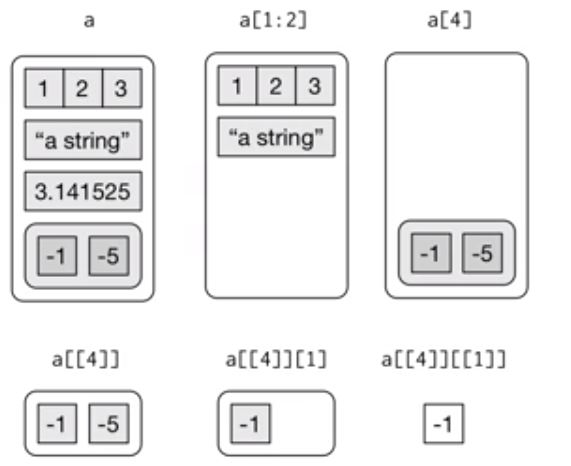
\includegraphics{images/list_example.JPG}
\caption{}
\end{figure}

\vspace{0.5cm}

\subsubsection{Named Lists}\label{named-lists}

\begin{Shaded}
\begin{Highlighting}[]
\NormalTok{my_named_list <-}\StringTok{ }\KeywordTok{list}\NormalTok{(}\DataTypeTok{title =} \StringTok{"statistics"}\NormalTok{, }\DataTypeTok{numbers =} \DecValTok{1}\OperatorTok{:}\DecValTok{10}\NormalTok{, }\DataTypeTok{data =} \OtherTok{TRUE}\NormalTok{)}
\NormalTok{my_named_list}
\end{Highlighting}
\end{Shaded}

\begin{verbatim}
## $title
## [1] "statistics"
## 
## $numbers
##  [1]  1  2  3  4  5  6  7  8  9 10
## 
## $data
## [1] TRUE
\end{verbatim}

\vspace{0.25cm}

We see the output for a named list is slightly different. Instead of
double brackets next to each component, there are now \texttt{\$} and
names of the variable. This will help you understand the structure of
data.frames (coming up next)!

\newpage

\section{Importing Data}\label{importing-data}

\begin{itemize}
\tightlist
\item
  Use the \textbf{Import Dataset} button in the \textbf{Environment}
  tab\\
\item
  Choose the \textbf{From CSV} option\\
\item
  Click on the \textbf{Browse} button\\
\item
  Direct the computer to where you saved the BlackfootFish data file,
  click \textbf{open}\\
\item
  It will bring up a preview of the data\\
\item
  Click on the \textbf{Import} button
\end{itemize}

Notice the code that outputs in the console (the bottom left square).
This is the code that you could have typed in the code chunk below to
import the data yourself. Copy and paste the code that was output in the
code chunk below.

\vspace{0.5cm}

\begin{Shaded}
\begin{Highlighting}[]
\CommentTok{# copy and paste the code that was used by R to import the data be careful to}
\CommentTok{# only copy the code that is next to the > signs!}
\end{Highlighting}
\end{Shaded}

\section{Structure of Data}\label{structure-of-data}

The data we will use is organized into data tables. When you imported
the BlackfootFish data into RStudio was saved as an object. You are able
to inspect the structure of the BlackfootFish object using functions
built in to \texttt{R} (no packages necessary).

Run the following code. What is output from each of the following
commands?

\vspace{0.25cm}

\begin{Shaded}
\begin{Highlighting}[]
\KeywordTok{class}\NormalTok{(BlackfootFish)  ## What is the object class of the data?}
\end{Highlighting}
\end{Shaded}

\begin{verbatim}
## [1] "data.frame"
\end{verbatim}

\begin{Shaded}
\begin{Highlighting}[]
\KeywordTok{dim}\NormalTok{(BlackfootFish)  ## What is the first number represent? What about the second number?}
\end{Highlighting}
\end{Shaded}

\begin{verbatim}
## [1] 18352     7
\end{verbatim}

\begin{Shaded}
\begin{Highlighting}[]
\KeywordTok{names}\NormalTok{(BlackfootFish)  ## What does this output refer to?}
\end{Highlighting}
\end{Shaded}

\begin{verbatim}
## [1] "trip"    "mark"    "length"  "weight"  "year"    "section" "species"
\end{verbatim}

\begin{Shaded}
\begin{Highlighting}[]
\KeywordTok{str}\NormalTok{(BlackfootFish)  ## What is the structure of the data?}
\end{Highlighting}
\end{Shaded}

\begin{verbatim}
## 'data.frame':    18352 obs. of  7 variables:
##  $ trip   : int  1 1 1 1 1 1 1 1 1 1 ...
##  $ mark   : int  0 0 0 0 0 0 0 0 0 0 ...
##  $ length : num  288 288 285 322 312 363 269 160 213 157 ...
##  $ weight : num  175 190 245 275 300 380 170 40 80 35 ...
##  $ year   : int  1989 1989 1989 1989 1989 1989 1989 1989 1989 1989 ...
##  $ section: chr  "Johnsrud" "Johnsrud" "Johnsrud" "Johnsrud" ...
##  $ species: chr  "RBT" "RBT" "RBT" "RBT" ...
\end{verbatim}

\newpage 

\begin{Shaded}
\begin{Highlighting}[]
\KeywordTok{summary}\NormalTok{(BlackfootFish)  ## What is the data type of each variable in our dataset?}
\end{Highlighting}
\end{Shaded}

\begin{verbatim}
##       trip            mark             length          weight      
##  Min.   :1.000   Min.   :0.00000   Min.   : 16.0   Min.   :   0.0  
##  1st Qu.:1.000   1st Qu.:0.00000   1st Qu.:186.0   1st Qu.:  65.0  
##  Median :2.000   Median :0.00000   Median :250.0   Median : 150.0  
##  Mean   :1.501   Mean   :0.09285   Mean   :262.3   Mean   : 246.2  
##  3rd Qu.:2.000   3rd Qu.:0.00000   3rd Qu.:330.0   3rd Qu.: 330.0  
##  Max.   :2.000   Max.   :1.00000   Max.   :986.0   Max.   :4677.0  
##                                                    NA's   :1796    
##       year        section            species         
##  Min.   :1989   Length:18352       Length:18352      
##  1st Qu.:1991   Class :character   Class :character  
##  Median :1996   Mode  :character   Mode  :character  
##  Mean   :1997                                        
##  3rd Qu.:2002                                        
##  Max.   :2006                                        
## 
\end{verbatim}

\begin{Shaded}
\begin{Highlighting}[]
\KeywordTok{typeof}\NormalTok{(BlackfootFish)  ## What is the storage mode of a data.frame?}
\end{Highlighting}
\end{Shaded}

\begin{verbatim}
## [1] "list"
\end{verbatim}

\vspace{0.5cm}

When we inspect dataframes, or other objects in \texttt{R}, there are
some general functions that are useful to check the content/structure of
the data. Here are some:

\begin{itemize}
\tightlist
\item
  size:

  \begin{itemize}
  \tightlist
  \item
    \texttt{dim(data)}: rows and columns\\
  \item
    \texttt{nrow(data)}: number of rows\\
  \item
    \texttt{ncol(data)}: number of columns
  \end{itemize}
\item
  content:

  \begin{itemize}
  \tightlist
  \item
    \texttt{head(data)}: first 6 rows\\
  \item
    \texttt{tail(data)}: last 6 rows\\
  \item
    \texttt{View(data)}: opens viewer window in separate tab
  \end{itemize}
\item
  names:

  \begin{itemize}
  \tightlist
  \item
    \texttt{colnames(data)}: column names of dataframe\\
  \item
    \texttt{rownames(data)}: row names of dataframe
  \end{itemize}
\item
  summary of content:

  \begin{itemize}
  \tightlist
  \item
    \texttt{str(data)}: structure of object and information about the
    columns\\
  \item
    \texttt{glimpse(data)}: similar information to \texttt{str}, but
    neater output\\
  \item
    \texttt{summary(data)}: summary statistics for each column
  \end{itemize}
\end{itemize}

\newpage

\section{Dataframes}\label{dataframes}

What is a dataframe? A dataframe is a type of \texttt{R} object and is
the \emph{de facto} structure of tabular data. You can create dataframes
by hand, but most of us do not use \texttt{R} to input our data by hand.
Instead, we import our data using \texttt{R} commands that read in
spreadsheets (\texttt{read.csv}, \texttt{read\_csv},
\texttt{read\_excel} etc.). A dataframe is a set of columns, where each
column is a vector. Thus, columns have the same data type \emph{within}
the column, but potentially different data types \emph{across} columns.

For example, the columns \texttt{trip}, \texttt{mark}, and \texttt{year}
are integers (whole numbers), \texttt{weight} and \texttt{length} are
numeric (numbers with decimals), and \texttt{section} and
\texttt{species} are characters.

\section{Extracting Data}\label{extracting-data}

If we were interested in accessing a specific variable in our dataset,
we can use the \texttt{\$} command. This command extracts the specified
variable (on the right of the \texttt{\$} sign) from the dataset. When
this is extracted, \texttt{R} views the variable as a vector of entries,
which is what the {[}1:18352{]} refers to.

\vspace{0.25cm}

\begin{Shaded}
\begin{Highlighting}[]
\NormalTok{years <-}\StringTok{ }\NormalTok{BlackfootFish}\OperatorTok{$}\NormalTok{year}
\NormalTok{## extracts year from the dataset and saves it into a new variable named year}

\KeywordTok{str}\NormalTok{(years)  ## using the new variable (remember case matters!)}
\end{Highlighting}
\end{Shaded}

\begin{verbatim}
##  int [1:18352] 1989 1989 1989 1989 1989 1989 1989 1989 1989 1989 ...
\end{verbatim}

\begin{Shaded}
\begin{Highlighting}[]
\NormalTok{## How would you determine how long the vector is?}
\end{Highlighting}
\end{Shaded}

\vspace{0.25cm}

Another method for accessing data in the dataset is using matrix
notation ({[}row, column{]}). If you look to your right in the
\textbf{Environment} window, you notice that RStudio tells you the
dimensions of the BlackfootFish data. You can (roughly) view the dataset
as a matrix of entries, with variable names for each of the columns. I
could instead use bracket notation to perform the same task as above,
using the following code.

\vspace{0.25cm}

\begin{Shaded}
\begin{Highlighting}[]
\NormalTok{years <-}\StringTok{ }\NormalTok{BlackfootFish[, }\DecValTok{5}\NormalTok{]}
\NormalTok{## This takes ALL rows of data but only the fifth column Same as years <-}
\NormalTok{## BlackfootFish[1:18352, 5]}

\KeywordTok{str}\NormalTok{(years)}
\end{Highlighting}
\end{Shaded}

\begin{verbatim}
##  int [1:18352] 1989 1989 1989 1989 1989 1989 1989 1989 1989 1989 ...
\end{verbatim}

\subsection{Practice:}\label{practice}

The following is a preview of the matrix \texttt{x}:

\begin{verbatim}
##      [,1] [,2] [,3] [,4]
## [1,]    1    2    3    4
## [2,]    5    6    7    8
## [3,]    9   10   11   12
## [4,]   13   14   15   16
\end{verbatim}

\vspace{0.25cm}

\textbf{Exercise 4:} What would be output if you entered:
\texttt{x{[}3,\ {]}}?

\vspace{0.25cm}

\textbf{Exercise 5:} What would you input to get an output of 4?

\vspace{1.5cm}

The following is a preview of the dataframe \texttt{df}:

\begin{verbatim}
##   x   y    z
## 1 H May 2010
## 2 N Oct 2015
## 3 T Mar 2018
## 4 W Aug 2017
## 5 V Feb 2019
\end{verbatim}

\vspace{0.25cm}

\textbf{Exercise 6:} What would you input to get an output of
\texttt{2015}? Can you think of two ways to do it?

\vspace{0.25cm}

\textbf{Exercise 7:} How would you pull off only columns \texttt{x} and
\texttt{z}? Can you think of two ways to do it?

\vspace{0.25cm}

\textbf{Exercise 8:} How would you modify the script below, to get an
output of \texttt{{[}1{]}\ 22\ 24}?

\vspace{0.25cm}

\begin{Shaded}
\begin{Highlighting}[]
\NormalTok{s <-}\StringTok{ }\KeywordTok{c}\NormalTok{(}\DecValTok{22}\NormalTok{, }\DecValTok{24}\NormalTok{, }\DecValTok{49}\NormalTok{, }\DecValTok{18}\NormalTok{, }\DecValTok{1}\NormalTok{, }\DecValTok{6}\NormalTok{)}
\NormalTok{s[]}
\end{Highlighting}
\end{Shaded}

\vspace{0.25cm}

\textbf{Exercise 9:} What would be output if you entered:
\texttt{s{[}3,\ {]}}?

\vspace{0.25cm}

\textbf{Exercise 10:} What would you input to get an output of
\texttt{{[}1{]}\ 22\ 49}?

\vspace{0.25cm}

\section{Changing Data Type}\label{changing-data-type}

Consider the variables species and section. These variables represent a
broader class of what we call categorical variables. In \texttt{R} there
are two ways to store this information, (1) as a series of
\texttt{character} strings, or (2) as a \texttt{factor}. In the early
days of coding in \texttt{R}, factors were more efficient than
characters, since you only need to store the level of the factor each
observation went with.

While factors are still useful in today's statistical analyses and data
visualizations, they can be tricky to deal with. When you convert a
variable to a factor, for many operations you will get different results
than for a character (McNamara \& Horton, 2017).

In these data section has two levels (Johnsrud and ScottyBrown) and
species has four levels (RBT, WCT, Bull, and Brown). If we want
\texttt{R} to view these variables as factors instead of characters, we
need to change their data type.

\vspace{0.25cm}

\begin{Shaded}
\begin{Highlighting}[]
\KeywordTok{unique}\NormalTok{(BlackfootFish}\OperatorTok{$}\NormalTok{species)  ## tells you the unique values of species}
\end{Highlighting}
\end{Shaded}

\begin{verbatim}
## [1] "RBT"   "WCT"   "Bull"  "Brown"
\end{verbatim}

\begin{Shaded}
\begin{Highlighting}[]
\KeywordTok{unique}\NormalTok{(BlackfootFish}\OperatorTok{$}\NormalTok{section)  ## tells you the unique values of section  }
\end{Highlighting}
\end{Shaded}

\begin{verbatim}
## [1] "Johnsrud"    "ScottyBrown"
\end{verbatim}

\begin{Shaded}
\begin{Highlighting}[]
\NormalTok{BlackfootFish}\OperatorTok{$}\NormalTok{speciesF <-}\StringTok{ }\KeywordTok{as.factor}\NormalTok{(BlackfootFish}\OperatorTok{$}\NormalTok{species)}
\NormalTok{## creates a new variable that is the factor version of species}
\NormalTok{BlackfootFish}\OperatorTok{$}\NormalTok{sectionF <-}\StringTok{ }\KeywordTok{as.factor}\NormalTok{(BlackfootFish}\OperatorTok{$}\NormalTok{section)}
\NormalTok{## creates a new variable that is the factor version of section}
\end{Highlighting}
\end{Shaded}

\newpage

There is also a function that will allow for you to specify the order of
the levels of a factor! As we saw before, the \texttt{as.factor}
function chooses the levels alphabetically. Suppose you would like for
the species to be in the following order: Bull, Brown, RBT, and WCT.

Using the \texttt{factor} function this would look like:

\vspace{0.25cm}

\begin{Shaded}
\begin{Highlighting}[]
\NormalTok{BlackfootFish}\OperatorTok{$}\NormalTok{speciesF <-}\StringTok{ }\KeywordTok{factor}\NormalTok{(BlackfootFish}\OperatorTok{$}\NormalTok{species, }
                                \DataTypeTok{levels =} \KeywordTok{c}\NormalTok{(}\StringTok{"Bull"}\NormalTok{, }\StringTok{"Brown"}\NormalTok{, }\StringTok{"RBT"}\NormalTok{, }\StringTok{"WCT"}\NormalTok{))}
\end{Highlighting}
\end{Shaded}

\subsection{Practice:}\label{practice-1}

\textbf{Exercise 11:} Year was saved as an integer data type (1989 -
2006), but we may want to consider it to be a categorical variable (a
factor). Write the \texttt{R} code to create a new variable called
\texttt{yearF} that is a factor of \texttt{year} (as you did with
section and species).

\vspace{0.25cm}

\textbf{Exercise 12:} Now, verify that \texttt{yearF} is viewed as a
categorical variable, with the same levels as \texttt{year}. (hint: you
have already used three functions that would do this for you)

\vspace{0.25cm}

The issue with factors, lies with if/when you want to change it back to
a number or character. In the code below I've decided that I don't want
year to be a factor and want to change it back to numeric. What happens
when I use the \texttt{as.numeric()} function on the yearF variable?

\vspace{0.25cm}

\begin{Shaded}
\begin{Highlighting}[]
\NormalTok{year_recover <-}\StringTok{ }\KeywordTok{as.numeric}\NormalTok{(BlackfootFish}\OperatorTok{$}\NormalTok{yearF)}

\NormalTok{ds <-}\StringTok{ }\KeywordTok{data.frame}\NormalTok{(}\DataTypeTok{original =}\NormalTok{ BlackfootFish}\OperatorTok{$}\NormalTok{yearF, }
                 \DataTypeTok{recovered =}\NormalTok{ year_recover)}
\KeywordTok{head}\NormalTok{(ds)}
\end{Highlighting}
\end{Shaded}

\begin{verbatim}
##   original recovered
## 1     1989         1
## 2     1989         1
## 3     1989         1
## 4     1989         1
## 5     1989         1
## 6     1989         1
\end{verbatim}

\section{Packages}\label{packages}

As we mentioned previously, \texttt{R} has many packages, which people
around the world work on to provide and maintain new software and new
capabilities for \texttt{R}. You will slowly accumulate a number of
packages that you use often for a variety of purposes. In order to use
the elements (data, functions) of the packages, you have to first
install the package (only once) and then load the package (every time).

We're going to install a few packages that are often used.

\begin{itemize}
\tightlist
\item
  Use the \textbf{Install} button in the \textbf{Packages} tab\\
\item
  Type in \texttt{devtools} and \texttt{tidyverse} into the blank line
  (separated by a comma)\\
\item
  Check the \textbf{Install dependencies} box\\
\item
  Click on the \textbf{Import} button
\end{itemize}

\newpage 

There will be a large amount of output coming out of the console. This
output is \texttt{R} trying to download the package(s) you requested by
contacting the mirror you chose for it to use when downloading (I chose
Northern Michigan University). Once the computer has downloaded the
packages, it will tell you that
``\texttt{The\ downloaded\ binary\ packages\ are\ in}'', followed by the
location of the files.

Now that the files are downloaded, we need to load them in order to use
them. The following code will load each package, please run it!

\vspace{0.25cm}

\begin{Shaded}
\begin{Highlighting}[]
\KeywordTok{library}\NormalTok{(devtools)}
\end{Highlighting}
\end{Shaded}

\begin{verbatim}
## Loading required package: usethis
\end{verbatim}

\begin{Shaded}
\begin{Highlighting}[]
\KeywordTok{library}\NormalTok{(tidyverse)}
\end{Highlighting}
\end{Shaded}

\begin{verbatim}
## ── Attaching packages ────────────────── tidyverse 1.2.1 ──
\end{verbatim}

\begin{verbatim}
## ✓ ggplot2 3.2.1     ✓ purrr   0.3.3
## ✓ tibble  2.1.3     ✓ dplyr   0.8.3
## ✓ tidyr   1.0.0     ✓ stringr 1.4.0
## ✓ ggplot2 3.2.1     ✓ forcats 0.4.0
\end{verbatim}

\begin{verbatim}
## ── Conflicts ───────────────────── tidyverse_conflicts() ──
## x dplyr::filter() masks stats::filter()
## x dplyr::lag()    masks stats::lag()
\end{verbatim}

\vspace{0.25cm}

Notice that when loading the \texttt{tidyverse} package that there is a
large amount of output. This output is telling you all of the other
packages that are loaded in the \texttt{tidyverse} package, as well as
the functions in the \texttt{tidyverse} package that overwrite (mask)
functions from base \texttt{R}.

This is the process you go through if you ever find packages that you
would like to use! Often packages that you install will need to be
updated. To update a package you can click on the ``Tools'' tab, then
click on ``Check for Package Updates''. This will bring up a window that
will list all of the packages that have newer versions than what you
have. Click on the packages that you wish to update, or click on the
``Select All'' button.

\section{Finding Help}\label{finding-help}

One of the chief reasons for \texttt{R}'s religious following is its
wonderful documentation. If you know a function does what you want (say
find the variance), but are not quite sure how it's spelled, what
arguments it takes, or what package it lives in, don't fret! The
\texttt{?} and \texttt{help()} commands are very powerful. For
functions, placing the \texttt{?} before the name, will tell \texttt{R}
to search for that name in all of the functions, in all of the packages
you have installed.

\begin{itemize}
\item
  If it finds \emph{one} \textbf{identical match}, it will display the
  help file for that function in the Help tab in the bottom-right
  corner.\\
\item
  If it finds \emph{more than one} \textbf{identical match}, it will
  display the functions, in their respective packages, that you have to
  choose from.\\
\item
  If it find \emph{no} \textbf{identical match}, it will tell you that
  ``\texttt{No\ documentation\ \ for\ \_\_\_\_\ in\ specified\ packages\ and\ libraries:,}''
  and suggests you use a \texttt{??} instead.

  \begin{itemize}
  \tightlist
  \item
    A \texttt{??} in front of the function name will search \textbf{all
    of \texttt{R}} for named functions similar to what you typed.\\
  \item
    The output will tell you what package the function is in, as well as
    the function's name (\texttt{package::function}).
  \end{itemize}
\end{itemize}

\vspace{0.25cm}

If you would like help on a particular package, say one that you just
downloaded, then you can use the same command(s) to get help. These
commands will load up a help page (in RStudio) in the Help pane. Each
help page is broken down into sections:

\begin{itemize}
\tightlist
\item
  Description: An extended description of what the function does.\\
\item
  Usage: The arguments of the function and their default values.\\
\item
  Arguments: An explanation of the object each argument is expecting.\\
\item
  Details: Any important details to be aware of.\\
\item
  Value: The object the function returns.\\
\item
  See Also: Any related functions that may be useful.\\
\item
  Examples: Some examples for how to use the function.
\end{itemize}

\section{Functions}\label{functions}

In \texttt{R} there are both functions that are built in (require no
package to be loaded), as well as functions that are housed within
specific packages. You have already used a few built in functions to
inspect the structure of the BlackfootFish data (\texttt{str},
\texttt{class}, \texttt{summary}). As we know, a function transforms an
input (potentially multiple) into an output. You have to provide
\texttt{R} with the inputs (arguments) required for the function to
generate an output. The argument(s) inside a function happen after the
\texttt{(} symbol. You know an object is a function when it is
immediately followed by a \texttt{(} and the corresponding closing
\texttt{)} comes after the arguments are complete. The output of a
function does not have to be numerical and it typically is not a single
number, it can be a set of things or a dataset.

Arguments describe the details of what a function is to do. Some
functions take arguments that are specified by the user, or, if left
undeclared, take on default values. These arguments are typically given
names (as seen in the help file), but the arguments are assumed to
follow the order the function expects if they are not named (also stated
in the help file). When naming an argument, the name of the argument is
followed by an \texttt{=} sign and then the value of the argument.
Notice that here we are using the \texttt{=} to declare what value each
argument is taking on, we \textbf{are not} creating a new variable with
that value assigned to it.

Suppose we wanted to create a vector of 10 zeros. To do this, we would
use both the \texttt{rep} function:

\vspace{0.25cm}

\begin{Shaded}
\begin{Highlighting}[]
\CommentTok{# ?rep}

\KeywordTok{rep}\NormalTok{(}\DecValTok{0}\NormalTok{, }\DataTypeTok{times =} \DecValTok{10}\NormalTok{)  ## repeating 0 three times}
\end{Highlighting}
\end{Shaded}

\begin{verbatim}
##  [1] 0 0 0 0 0 0 0 0 0 0
\end{verbatim}

\begin{Shaded}
\begin{Highlighting}[]
\KeywordTok{rep}\NormalTok{(}\DataTypeTok{times =} \DecValTok{10}\NormalTok{, }\DecValTok{0}\NormalTok{)  ## switching order of arguments}
\end{Highlighting}
\end{Shaded}

\begin{verbatim}
##  [1] 0 0 0 0 0 0 0 0 0 0
\end{verbatim}

\begin{Shaded}
\begin{Highlighting}[]
\KeywordTok{rep}\NormalTok{(}\DecValTok{0}\NormalTok{, }\DecValTok{10}\NormalTok{)  ## no named arguments}
\end{Highlighting}
\end{Shaded}

\begin{verbatim}
##  [1] 0 0 0 0 0 0 0 0 0 0
\end{verbatim}

\begin{Shaded}
\begin{Highlighting}[]
\KeywordTok{rep}\NormalTok{(}\DecValTok{10}\NormalTok{, }\DecValTok{0}\NormalTok{)  ## not what we wanted!}
\end{Highlighting}
\end{Shaded}

\begin{verbatim}
## numeric(0)
\end{verbatim}

\vspace{0.25cm}

Now let's look over some other functions that are often used:

\vspace{0.25cm}

\begin{Shaded}
\begin{Highlighting}[]
\KeywordTok{mean}\NormalTok{(BlackfootFish}\OperatorTok{$}\NormalTok{weight)  ## takes a numerical input, but there are NA's in our data}

\KeywordTok{mean}\NormalTok{(BlackfootFish}\OperatorTok{$}\NormalTok{weight, argument here}\OperatorTok{!}\StringTok{ }\NormalTok{)  ## add in the argument that removes the NA's}

\KeywordTok{median}\NormalTok{(BlackfootFish}\OperatorTok{$}\NormalTok{species) ## gives an error because the input is not the correct data type  }

\KeywordTok{cor}\NormalTok{(BlackfootFish}\OperatorTok{$}\NormalTok{length, BlackfootFish}\OperatorTok{$}\NormalTok{weight) ## takes multiple inputs separated by a comma}

\NormalTok{## Does cor have an option to remove NA's?}
\end{Highlighting}
\end{Shaded}

\vspace{0.25cm}

As seen in the functions above, some functions have \emph{optional}
arguments. If they are not specified by the user, then they take on
their default value (\texttt{FALSE} for \texttt{na.rm}). These options
control the behavior of the functions, such as whether it
includes/excludes NA values.

\section{Cleaning Data}\label{cleaning-data}

In many instances, you will deal with data that are not ``clean''. Based
on the output we received from the \texttt{mean()} function, we know
that there are NA's in the BlackfootFish data, possibly across a variety
of variables. Before we used \texttt{na.rm} as an option to remove NA's
\emph{within} a function, but the \texttt{na.omit} function takes a
dataframe and removes any NA's from that dataset. Based on the output
below, how many rows in the BlackfootFish data have an NA present?

\vspace{0.5cm}

\begin{Shaded}
\begin{Highlighting}[]
\KeywordTok{dim}\NormalTok{(BlackfootFish)  ## gives the dimensions of the dataset in (row, column) format  }
\end{Highlighting}
\end{Shaded}

\begin{verbatim}
## [1] 18352    10
\end{verbatim}

\begin{Shaded}
\begin{Highlighting}[]
\KeywordTok{dim}\NormalTok{(}\KeywordTok{na.omit}\NormalTok{(BlackfootFish))}
\end{Highlighting}
\end{Shaded}

\begin{verbatim}
## [1] 16556    10
\end{verbatim}

\begin{Shaded}
\begin{Highlighting}[]
\NormalTok{## na.omit takes dataframes, matricies, and vectors and returns the object with}
\NormalTok{## incomplete cases removed (NA's removed)}
\end{Highlighting}
\end{Shaded}

\vspace{0.5cm}

\textbf{Remark:} The computer is using an algorithm to return a dataset
with no NA values anywhere in it. This algorithm goes through every row
of the dataset and (roughly) has the following steps,

\begin{itemize}
\tightlist
\item
  Inspect the row to see if there is an NA anywhere in that row\\
\item
  If there is an NA in that row, the logical (\texttt{is.na}) evaluates
  to TRUE, and the row is deleted\\
\item
  If there is not any NA's in that row, the logical evaluates to FALSE,
  and the row is retained\\
\item
  Once it has stepped through every row, the function outputs the
  ``cleaned'' dataframe
\end{itemize}

\section{Subsetting Data}\label{subsetting-data}

If we wish to remove all of the NA's from the dataset, we can simply use
the \texttt{na.omit} command from above. We can save the new ``clean''
dataset under a new name (creating a new object) or under the same name
as before (replacing the old object with the new object).

\vspace{0.25cm}

\begin{Shaded}
\begin{Highlighting}[]
\NormalTok{BlackfootFish_clean <-}\StringTok{ }\KeywordTok{na.omit}\NormalTok{(BlackfootFish)}
\NormalTok{## Creates a new dataframe, where the NA's have all been removed}
\end{Highlighting}
\end{Shaded}

\vspace{0.25cm}

\section{Data Visualization}\label{data-visualization}

There are many different genres of data graphics, with many different
variations on each genre. Here are some commonly encountered kinds:

\begin{itemize}
\tightlist
\item
  \textbf{scatterplots}: showing relationships between two quantitative
  variables\\
\item
  \textbf{distributions}: showing distributions of a single quantitative
  variable\\
\item
  \textbf{bar charts}: displaying frequencies or densities of a single
  categorical variable
\end{itemize}

\subsection{Scatterplots}\label{scatterplots}

The main purpose of the scatterplot is to show the relationship between
two variables across several or many cases. Most often, there is a
Cartesian coordinate system in which the x-axis represents one variable
and the y-axis the second variable.

\vspace{0.25cm}

\begin{Shaded}
\begin{Highlighting}[]
\CommentTok{#?plot()}
\KeywordTok{plot}\NormalTok{(length }\OperatorTok{~}\StringTok{ }\NormalTok{weight, }
     \DataTypeTok{data =}\NormalTok{ BlackfootFish_clean) }
\end{Highlighting}
\end{Shaded}

\begin{center}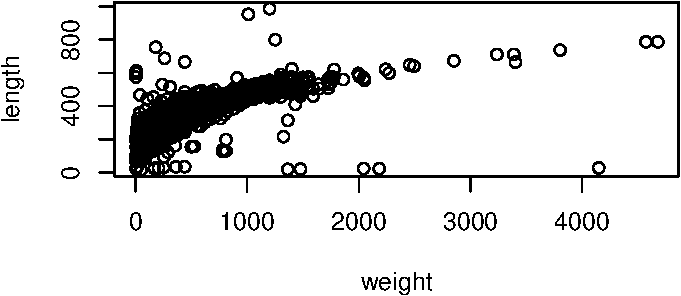
\includegraphics{RTutorial_files/figure-latex/scatter1-1} \end{center}

\newpage

\begin{Shaded}
\begin{Highlighting}[]
\KeywordTok{plot}\NormalTok{(length }\OperatorTok{~}\StringTok{ }\NormalTok{weight, }
     \DataTypeTok{data =}\NormalTok{ BlackfootFish_clean, }
     \DataTypeTok{xlab =} \StringTok{"Weight (gm)"}\NormalTok{, ## adding in axis labels}
     \DataTypeTok{ylab =} \StringTok{"Length (cm)"}\NormalTok{, }
     \DataTypeTok{las =} \DecValTok{1}\NormalTok{ ## changing orientation of axis labels}
\NormalTok{     ) }
\end{Highlighting}
\end{Shaded}

\begin{center}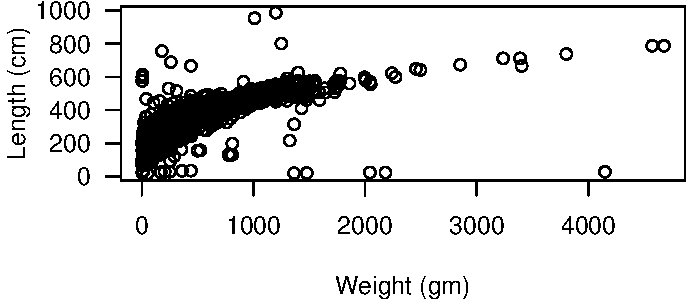
\includegraphics{RTutorial_files/figure-latex/scatter2-1} \end{center}

\subsection{Distribution}\label{distribution}

A histogram shows how many observations fall into a given range of
values of a variable.

\vspace{0.25cm}

\begin{Shaded}
\begin{Highlighting}[]
\KeywordTok{hist}\NormalTok{(BlackfootFish_clean}\OperatorTok{$}\NormalTok{length)}
\end{Highlighting}
\end{Shaded}

\begin{center}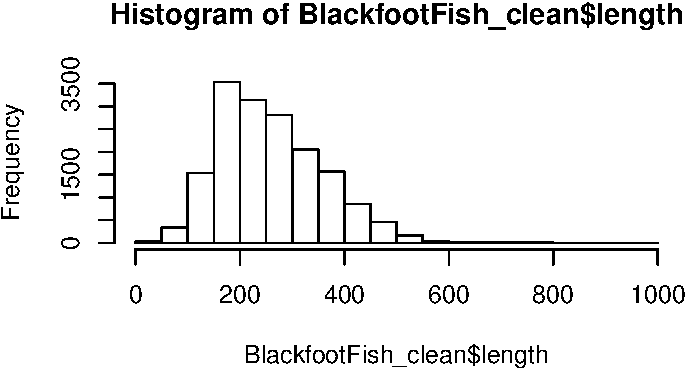
\includegraphics{RTutorial_files/figure-latex/hist1-1} \end{center}

\newpage

\begin{Shaded}
\begin{Highlighting}[]
\KeywordTok{hist}\NormalTok{(BlackfootFish_clean}\OperatorTok{$}\NormalTok{length, }
     \DataTypeTok{freq =}\NormalTok{ F) ## converts to a density plot (area adds to 1) }
\end{Highlighting}
\end{Shaded}

\begin{center}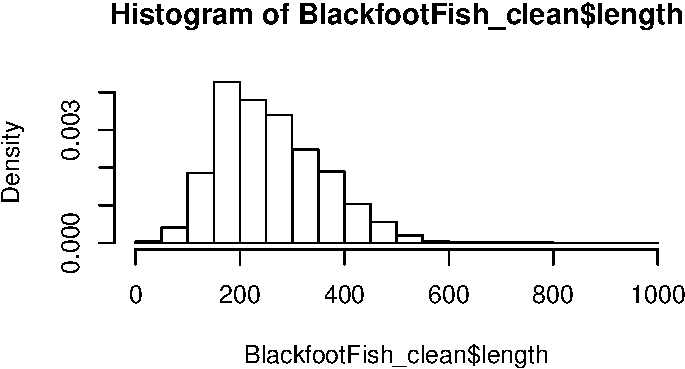
\includegraphics{RTutorial_files/figure-latex/hist2-1} \end{center}

\vspace{0.25cm}

\begin{Shaded}
\begin{Highlighting}[]
\NormalTok{## Does freq need to be named?}
\KeywordTok{hist}\NormalTok{(BlackfootFish_clean}\OperatorTok{$}\NormalTok{length, }\OtherTok{FALSE}\NormalTok{)}
\NormalTok{## Why is there an error about the 'number of breaks'?}
\end{Highlighting}
\end{Shaded}

\vspace{0.25cm}

\begin{Shaded}
\begin{Highlighting}[]
\KeywordTok{hist}\NormalTok{(BlackfootFish_clean}\OperatorTok{$}\NormalTok{length, }
     \DataTypeTok{freq =}\NormalTok{ F, }
     \DataTypeTok{xlab =} \StringTok{"Length"}\NormalTok{, ## adds x-axis label }
     \DataTypeTok{main =} \StringTok{"Fish Lengths in Blackfoot River"}\NormalTok{ ## adds title to plot}
\NormalTok{     ) }
\end{Highlighting}
\end{Shaded}

\begin{center}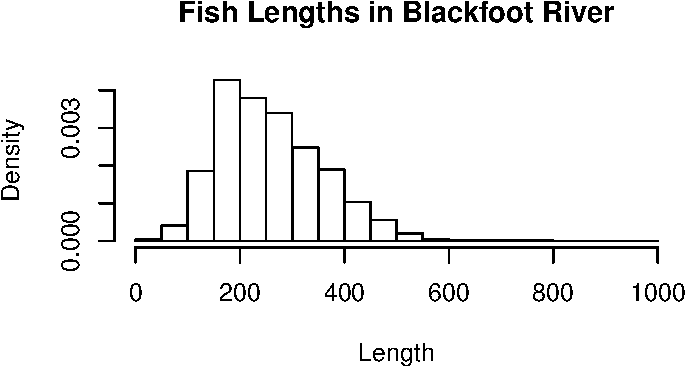
\includegraphics{RTutorial_files/figure-latex/hist3-1} \end{center}

\newpage

\begin{Shaded}
\begin{Highlighting}[]
\KeywordTok{hist}\NormalTok{(BlackfootFish_clean}\OperatorTok{$}\NormalTok{length, }
     \DataTypeTok{freq =}\NormalTok{ F, }
     \DataTypeTok{nclass =} \DecValTok{50}\NormalTok{, ## changes the number of bins }
     \DataTypeTok{xlab =} \StringTok{"Length"}\NormalTok{, }
     \DataTypeTok{main =} \StringTok{"Fish Lengths in the Blackfoot River"}\NormalTok{, }
     \DataTypeTok{las =} \DecValTok{1}\NormalTok{ ## changes orientation of axis labels}
\NormalTok{     ) }
\end{Highlighting}
\end{Shaded}

\begin{center}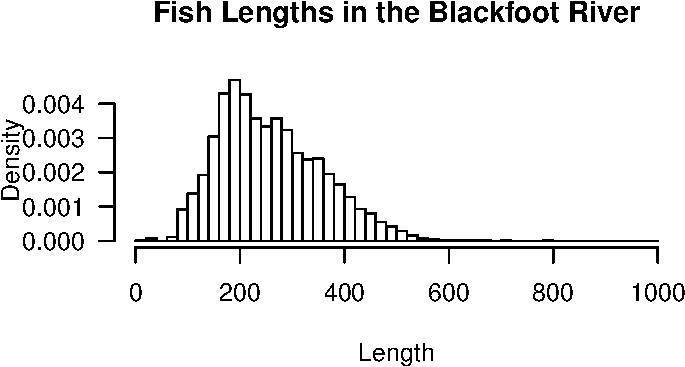
\includegraphics{RTutorial_files/figure-latex/hist4-1} \end{center}

\subsection{Side-by-Side Boxplots}\label{side-by-side-boxplots}

The familiar boxplot is effective when the objective is to compare the
distribution of a quantitative variable across different levels of a
categorical variable.

\vspace{0.25cm}

\begin{Shaded}
\begin{Highlighting}[]
\NormalTok{## What other options are available to add to your boxplot?}
\KeywordTok{boxplot}\NormalTok{(weight }\OperatorTok{~}\StringTok{ }\NormalTok{species, }
        \DataTypeTok{data =}\NormalTok{ BlackfootFish_clean)}
\end{Highlighting}
\end{Shaded}

\begin{center}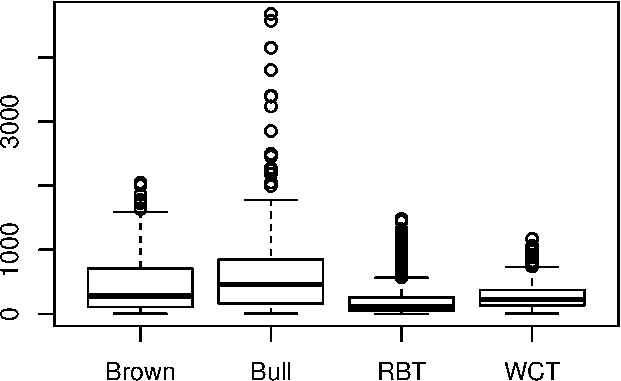
\includegraphics{RTutorial_files/figure-latex/boxplot-1} \end{center}

\vspace{0.25cm}

\subsection{Bar Charts}\label{bar-charts}

Bar charts are an effective way to compare the frequencies of levels of
a categorical variable.

\vspace{0.25cm}

\begin{Shaded}
\begin{Highlighting}[]
\NormalTok{section <-}\StringTok{ }\KeywordTok{table}\NormalTok{(BlackfootFish_clean}\OperatorTok{$}\NormalTok{section)}
\NormalTok{## tables the number of fish that were caught in each section}

\KeywordTok{barplot}\NormalTok{(section, }
        \DataTypeTok{xlab =} \StringTok{"Section"}\NormalTok{, ## adds axis labels to plot }
        \DataTypeTok{ylab =} \StringTok{"Number of Fish"}\NormalTok{, }
        \DataTypeTok{main =} \StringTok{"Fish Caught by Section"}\NormalTok{, ## adds title to plot}
        \DataTypeTok{las =} \DecValTok{1}\NormalTok{, ## changes orientation of axis labels}
        \DataTypeTok{col =} \StringTok{"blue"}\NormalTok{, ## specifies what color the bars should be}
        \DataTypeTok{ylim =} \KeywordTok{c}\NormalTok{(}\DecValTok{0}\NormalTok{, }\DecValTok{12000}\NormalTok{) ## specifies what range of y-values to plot}
\NormalTok{        )}
\end{Highlighting}
\end{Shaded}

\begin{center}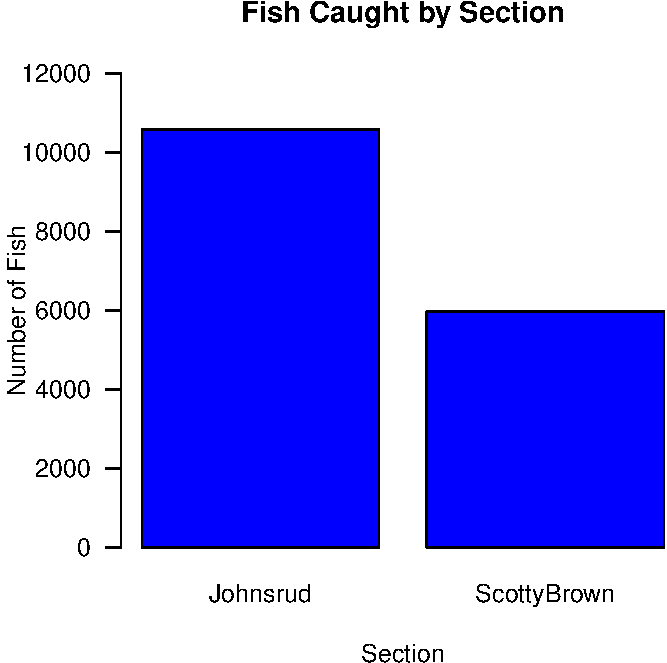
\includegraphics{RTutorial_files/figure-latex/bar-1} \end{center}

\vspace{0.25cm}

\subsection{Practice}\label{practice-2}

\textbf{Exercise 13:} Using statistics or graphics, which year in our
dataset had the most fish caught?

\vspace{2cm}

\textbf{Exercise 14:} Make a boxplot of the fish weights over the
different years in the dataset.

\newpage 

\section{Terminology Used in
Workshop}\label{terminology-used-in-workshop}

\begin{itemize}
\item
  \emph{Command}: A command is what \texttt{R} executes. In an
  \texttt{R} script file (script.R), commands are automatically implied,
  as this type of file does not accept text, only in comments. In an Rnw
  (Markdown) file (report.Rnw), commands are delineated between three
  ticks on the top (\texttt{\{r\})\ and\ three\ ticks\ (}) on the
  bottom.
\item
  \emph{Comment}: Helpful text added into a script environment. Comments
  can be used to describe functions, processes, a train of thought, so
  that when you return to your code, tomorrow or next year, you are able
  to understand the purpose of each line of code!
\item
  \emph{Object}: A variable created in \texttt{R}, to be used elsewhere
  in the code. Objects can be a variety of things, such as scalars (x
  \textless{}- 3), vectors (x \textless{}- c(1, 2, 3, 4, 5)), matrices,
  and dataframes, to name a few.
\item
  \emph{Assignment Arrow}: The assignment arrow \texttt{\textless{}-} is
  used to assign values on the right to the objects on the left (x
  \textless{}- 1). For historical reasons, you can also use \texttt{=}
  for assignments, but not everywhere. Because of these slight
  differences, it is recommended to \emph{always} use assignment arrows
  for assignment.
\item
  \emph{Class}: Most \texttt{R} objects have a class attribute, a
  character vector giving the names of the classes from which the object
  inherits. Examples of classes are numeric, factor, integer, character,
  dataframe, matrix, list.
\item
  \emph{Vector}: A vector is a list of entries, all sharing the same
  class. A vector has only one dimension, so data extraction uses only a
  single entry in brackets (e.g.~x{[}3{]}). You can create vectors of
  characters (c(``a'', ``b'', ``c'')), vectors of numbers (c(1, 2, 3)),
  to name a few.
\item
  \emph{Matrix}: Similar to what you may have seen in a mathematics
  class, a matrix is an object with rows and columns, where every entry
  in the matrix must be a number.
\item
  \emph{List}: A generic vector, which contains other objects. A list
  can contain a variety of different classes of objects,
  e.g.~characters, vectors, data.frames, matrices, or outputs from a
  model! A data.frame is a special type of list where the components are
  vectors and they all have the same length.
\item
  \emph{Dataframe}: A dataframe is a collection of variables. Dataframes
  share many of the properties of matrices, where you are able to
  extract elements using bracket ({[}{]}) notation, and lists, where you
  are able to extract columns using \texttt{\$}. Dataframes are used as
  the fundamental data structure by most of \texttt{R}'s statistical
  modeling software.
\item
  \emph{Argument}: Input(s) into a function, so that an output is
  created. Most functions take named arguments (e.g.~data =
  BlackfootFish) and the order of the arguments is assumed to follow the
  order found in the function's help file. When using a named argument
  in a function, the name comes first, followed by an = sign, then the
  input.
\item
  \emph{Logical Value}: TRUE and FALSE value(s) that can be used to turn
  off/on options in functions and plots, and also to manipulate data.
\end{itemize}

\newpage

\section{Workshop Materials \& Recordings
Available:}\label{workshop-materials-recordings-available}

\begin{itemize}
\item
  through RStudio Cloud at: \url{http://bit.ly/introduction-R}
\item
  through Allison's personal website at:
  \url{http://www.math.montana.edu/allison_theobold}
\item
  through the MSU Library YouTube channel:
  \url{https://www.youtube.com/watch?v=W6E3hpcoUkQ\&feature=youtu.be}
\end{itemize}

\section{\texorpdfstring{How to Learn More About
\texttt{R}}{How to Learn More About R}}\label{how-to-learn-more-about-r}

This material is intended to provide you with an introduction to using
\texttt{R} for scientific analyses of data. The best way for you to
continue to learn more about \texttt{R} is to use it in your research!
This may sound daunting, but writing \texttt{R} scripts is the best way
to become familiar with the syntax. This will help you progress through
more advanced operations, such as cleaning your data, using statistical
methods, or creating graphics.

The best place to start is playing around with the code from today's
workshop. Change parts of the code and see what happens! Better yet, use
the code from the workshop to investigate your own data!

\vspace{4cm}

Workshop build on: 2020-01-05 18:13:41


\end{document}
